% !TeX root = skripta-konstitutivni-vztahy.tex
% !TeX lastmodified = 2018-10-30

\subsection{Model Arruda-Boyce}\label{sec:arruda-boyce}
Tento model\footnote{Arruda EM, Boyce  MC: A three-dimensional constitutive model for large stretch behavior of rubber elastic materials. J. Mechanics and Physics of Solids, 1993, Vol. 41/2, pp. 389-412.} na rozdíl od předchozích modelů ryze fenomenologických vychází ze struktury materiálu, tvořené vláknitými zvlněnými řetězci makromolekul elastomeru.
Při jejich protažení dochází postupně k~jejich napřimování a~tím ke zvyšování tuhosti elastomeru -- deformačnímu zpevnění.
Protože řetězce jsou v~prostoru náhodně uspořádány (izotropní materiál), vyžaduje vyčíslení jejich příspěvku k~deformační energii všesměrovou 3D integraci (přes kouli).
Pro zjednodušení byla hledána taková uspořádání vláken, která při zachování symetrie podle hlavních materiálových rovin umožní jednodušší vyčíslení.
Dříve navržená zjednodušení (třířetězcový model krychlový, čtyřřetězcový model tetraedrický) tyto požadavky nesplňovala.

\begin{figure}[H]
	\centering
	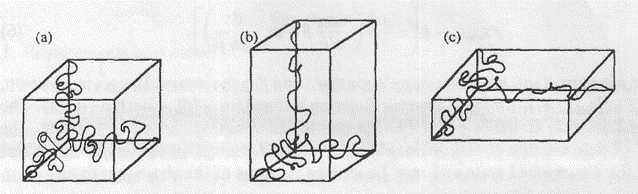
\includegraphics{triretezcovy-model-krychlovy}
	\caption{Třířetězcový model krychlový}
	\label{fig:triretezcovy-model-krychlovy}
\end{figure}

\begin{figure}[H]
	\centering
	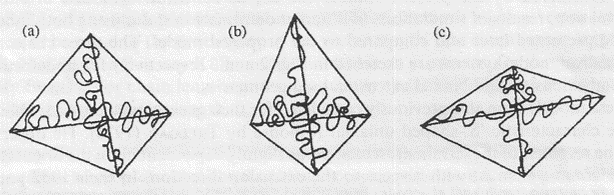
\includegraphics{ctyrretezcovy-model-tetraedricky}
	\caption{Čtyřřetězcový model tetraedrický}
	\label{fig:ctyrretezcovy-model-tetraedricky}
\end{figure}

Model Arruda-Boyce zavádí hexagonální buňku (krychli) s~rohy propojenými s~jejím středem pomocí osmi molekulárních řetězců -- proto někdy nazýván \uv{8-chain model}.

\begin{figure}[H]
	\centering
	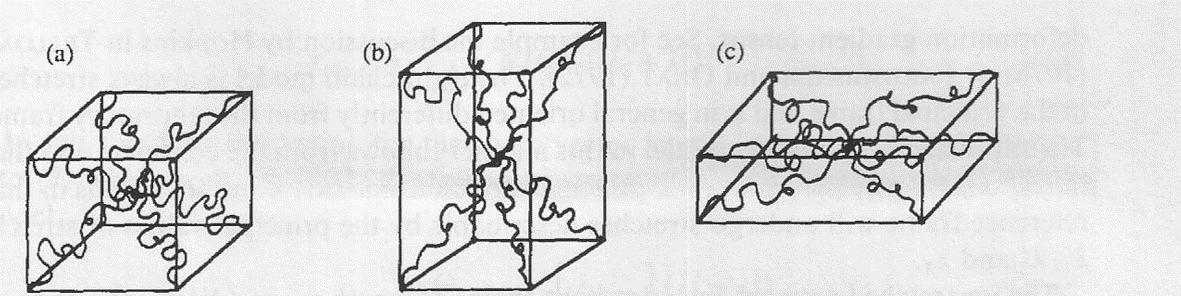
\includegraphics[width=0.75\linewidth]{osmiretezcovy-model-krychlovy}
	\caption{Osmiřetěžcový model krychlovy}
	\label{fig:osmiretezcovy-model-krychlovy}
\end{figure}

Molekulární řetězce elastomerů nejsou na rozdíl od krystalických materiálů spojeny kovalentními vazbami a~uplatňuje se u~nich jiný deformační mechanismus.
Vhodným modelem je řetězec tuhých článků vzájemně spojených rotačními vazbami, které minimalizují ohybovou tuhost řetězce.
Pak je jeho tvar výsledkem náhodných tepelných fluktuací a~o~pravděpodobnosti určitého tvaru molekulárního řetězce rozhoduje entropie -- jedná se o entropickou elasticitu.

Pro protažení řetězce definované obvyklým způsobem
\begin{equation}
	\lambda_\text{chain} = \frac{r_\text{chain}}{r_0}
\end{equation}
kde $r_0 = l \sqrt{N}$ je počáteční délka řetězce, daná statisticky délkou článku řetězce $l$ a~počtem článků $N$.
Limitní délka řetězce a~limitní protažení řetězce je pak
\begin{equation}
	r_L = l N
	\qquad
	\lambda_L = \frac{r_L}{r_0} = \sqrt{N}
\end{equation}
Model vychází z předpokladu afinní deformace (deformace řetězců-vláken je identická s~deformací okolní matrice).

Použijeme-li pro tvar řetězce Gaussovu statistiku, dostaneme pro model Neo-Hooke energii napjatosti ve tvaru:
\begin{equation}
	W = \frac{1}{2} G (\bar{I}_1 - 3)
	= \frac{1}{2} G \left(\lambda_1^2 + \lambda_2^2 + \lambda_3^2 - 3\right)
\end{equation}
kde
\begin{description}
	\item[{$G = n k_B T$}] je počáteční modul pružnosti ve smyku,
	\item[$n$] je hustota řetězce (počet řetězců v jednotkovém objemu)
	\item[$k_B$] je Boltzmannova konstanta,
	\item[$T$] je absolutní teplota.
\end{description}

Použitím Langevinovy statistiky dostaneme konfigurační entropii pro délku řetězce $r_\text{chain}$:
\begin{equation}
	S_\text{chain} = k_B \left\{c - N\left[\frac{r_\text{chain}}{N l} \beta + \ln\left(\frac{\beta}{\sinh(\beta)}\right) \right]\right\}
\end{equation}
kde $c$ je konstanta a~$\beta$ je inverzní Langevinova funkce definovaná vztahem
\begin{equation}
	\beta = \Im\left(\frac{r_\text{chain}}{N l}\right)
\end{equation}
pro
\begin{equation}
	\Im(\beta) = \coth(\beta) - \frac{1}{\beta}
\end{equation}

Použití Langevinovy statistiky umožňuje správně započítat limitní protažení strukturních řetězců $\lambda_L$. Deformační práce při izotermickém ději je pak úměrná změně entropie při protažení řetězců a~dá se vyjádřit následovně
\begin{equation}\label{eq:deformacni-prace-izotermickeho-deje}
	W = n k_B T N \left[\frac{r_\text{chain}}{N l} \beta + \ln\left(\frac{\beta}{\sinh(\beta)}\right) \right]
	= G \lambda_L \left\{ \lambda_\text{chain} \beta - \lambda_L \ln\left[ \frac{\sinh(\beta)}{\beta} \right] \right\}
\end{equation}

Složky napětí dostaneme standardním způsobem derivací podle složek deformačního tenzoru. Protože materiál je nestlačitelný, figuruje ve vztahu hydrostatický tlak jako další proměnná (Lagrangeův multiplikátor), která se musí určit z~okrajových podmínek.

Deformace různě orientovaných řetězců je při každém deformačním stavu různá, takže pro určení celkové deformační práce je nutné pro každý takový stav provádět integraci přes distribuci různě orientovaných řetězců.
Při deformaci dochází k~rotaci jednotlivých řetězců, takže pro určení jejich protažení (stretch tensor) je třeba provést polární dekompozici tenzoru deformačního gradientu a~poté určit hlavní souřadnice tenzoru protažení.
Derivací této práce podle hlavních protažení (hlavní složky tenzoru protažení) dostaneme 1.~Piola-Kirchhoffovo napětí a~následně skutečné napětí $\sigma_i$:
\begin{equation}
	\sigma_i = \lambda_i \frac{\diff W}{\diff \lambda_i} + p
\end{equation}
kde $p$ je Lagrangeův multiplikátor s~fyzikálním významem tlaku, který se určí z~okrajových podmínek. Ten lze eliminovat vyjádřením rozdílu hlavních napětí
\begin{equation}
	\sigma_1 - \sigma_2 = \lambda_1 \frac{\diff W}{\diff \lambda_1} - \lambda_2 \frac{\diff W}{\diff \lambda_2}
\end{equation}

Výhodou modelu je kromě (kubické) symetrie podle všech hlavních rovin, že všechny řetězce jsou při jakémkoli deformačním stavu protahovány (dáno podmínkou nestlačitelnosti materiálu).

V~nedeformovaném stavu je délka kteréhokoli z~řetězců v krychli o~hraně $a_0$ dána vztahem:
\begin{equation}
	2 r_0 = \sqrt{3 a_0^2} = \sqrt{3} a_0
	\quad\Rightarrow\quad
	r_0 = \frac{\sqrt{3}}{2} a_0
\end{equation}
Vektorově je ho možné napsat v~hlavním souřadnicovém systému tenzoru protažení (konkrétně pro řetězec směřující do 1.~kvadrantu):
\begin{equation}
	\vec{r}_0 = \frac{a_0}{2} \vec{i} + \frac{a_0}{2} \vec{i} + \frac{a_0}{2} \vec{k}
\end{equation}

V~deformovaném stavu bude vektorový zápis:
\begin{equation}
	\vec{r}_\text{chain} = \lambda_1 \frac{a_0}{2} \vec{i} + \lambda_2 \frac{a_0}{2} \vec{i} + \lambda_3 \frac{a_0}{2} \vec{k}
\end{equation}
a~velikost vektoru řetězce v~deformovaném stavu bude
\begin{equation}
	r_\text{chain} = \frac{a_0}{2} \sqrt{\lambda_1^2 + \lambda_2^2 + \lambda_3^2}
\end{equation}
Pak protažení tohoto řetězce je
\begin{equation}\label{eq:protazeni-retezce}
	\lambda_\text{chain}
	= \frac{r_\text{chain}}{r_0}
	= \frac{\sqrt{\lambda_1^2 + \lambda_2^2 + \lambda_3^2}}{\sqrt{3}}
	= \sqrt{\frac{I_1}{3}}
\end{equation}
Dosazením (\ref{eq:protazeni-retezce}) do (\ref{eq:deformacni-prace-izotermickeho-deje}) dostaneme energii $W$ jako funkci $I_1$.

Aplikujeme-li nyní pro popis náhodné prostorové distribuce řetězců polynomický rozvoj inverzní Langevinovy funkce a~použijeme jeho prvních pět členů, dostaneme deformační energii:
\begin{multline}
	W
	= n k_B T \left[ \frac{1}{2} (\bar{I}_1-3) + \frac{1}{20 N} (\bar{I}_1^2-9) + \frac{11}{1050 N^2} (\bar{I}_1^3-27) \right.\\
	\left. + \frac{19}{7000 N^3} (\bar{I}_1^4-81) + \frac{519}{673750 N^4} (\bar{I}_1^5-243) \right]
\end{multline}

Dosazením dříve odvozeného vztahu $\alpha_L = \sqrt{N} \Rightarrow N = \lambda_L^2$ a~přidáním členu popisujícího energii objemové části deformace dostaneme výsledný vztah:
\begin{multline}
	W
	= G \left[ \frac{1}{2} (\bar{I}_1-3) + \frac{1}{20 \lambda_L^2} (\bar{I}_1^2-9) + \frac{11}{1050 \lambda_L^4} (\bar{I}_1^3-27) \right.\\
	\left. + \frac{19}{7000 \lambda_L^6} (\bar{I}_1^4-81) + \frac{519}{673750 \lambda_L^8} (\bar{I}_1^5-243) \right]
	+ \frac{1}{d} \left(\frac{J^2 - 1}{2} - \ln(J)\right)
\end{multline}
kde $d=\frac{2}{K}$.

Pro $\lambda_L \rightarrow \infty$ se model redukuje na model \hyperref[sec:neo-hooke]{Neo-Hooke}.

\subsubsection{Výhody modelu Arruda-Boyce}
\begin{itemize}
	\item Model je téměř izotropní (nepatrná závislost na orientaci reprezentativní krychle resp. řetězců vůči směru zatížení) a~má vysokou míru symetrie vůči hlavním rovinám protažení.
	\item V~každém zatěžovacím stavu se všechny řetězce podílejí na přenosu zatížení. Jejich protažení se vzájemně liší a~díky jejich natáčení limitní protažení struktury přesahuje limitní protažení řetězce $\lambda_L$, které je však rozhodující pro zpevňování v~kterémkoli směru a~deformačním modu.
	\item Model má pouze 2 materiálové parametry pro deviátorovou část a~je schopen popsat zatěžovací křivku s~inflexí (zpevňující).
	\item Na rozdíl od fenomenologických modelů mají oba parametry jasně definovaný fyzikální význam.
	\item Díky strukturní povaze modelu má výbornou predikční schopnost; i~když použijeme pro určení jeho parametrů jen určitý typ napjatosti (např. jednoosou tahovou), dává rozumné výsledky i~pro jiné typy napjatosti.
\end{itemize}

\begin{figure}[H]
	\centering
	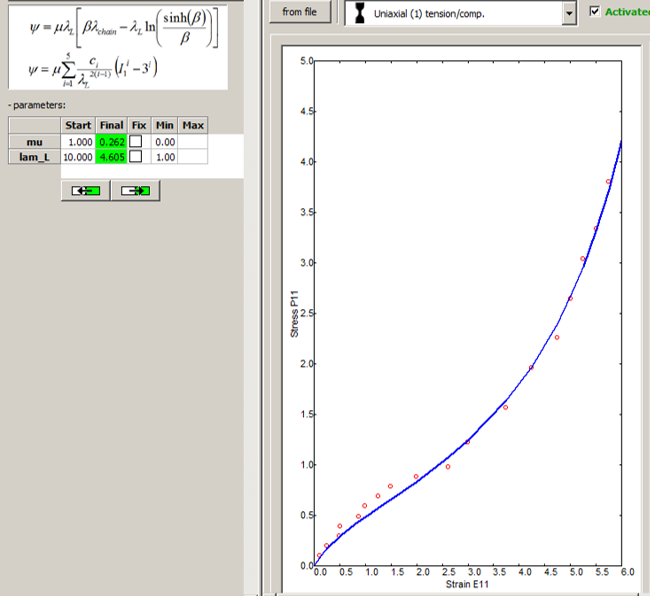
\includegraphics[width=0.5\linewidth]{aproximace-arruda-boyce}
	\caption{Proložení reálné experimentální křivky modelem Arruda-Boyce}
	\label{fig:aproximace-arruda-boyce}
\end{figure}
